\chapter{Utilities}
\label{ch:utilities}

%%%%%%%%%%%%%%%%%%
\section{Overview}

The functionalities shared between all the components of LAR
are defined in here.

@O lib/jl/utilities.jl
@{@< Utilities @>
@}

\subsection{Tests}
As usual every function has some unit tests.

@O test/jl/utilities.jl
@{using Base.Test
using LARLIB

@< Utilities tests @>
@}


%%%%%%%%%%%%%%%%%%%%%%%%
\section{Bounding boxes}
\label{sec:bboxes}

Bounding boxes are essential in many steps of many
algorithms in LAR. Here we present a method for building
and performing containment tests on n-dimensional 
axis aligned bounding boxes.

@D Utilities
@{function bbox(vertices::Verts)
    minimum = mapslices(x->min(x...), vertices, 1)
    maximum = mapslices(x->max(x...), vertices, 1)
    minimum, maximum
end

function bbox_contains(container, contained)
    b1_min, b1_max = container
    b2_min, b2_max = contained
    all(map((i,j,k,l)->i<=j<=k<=l, b1_min, b2_min, b2_max, b1_max))
end
@}

\subsection{Tests}
\begin{figure}[h]
    \centering
    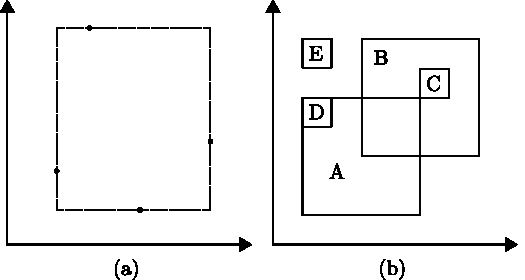
\includegraphics{./img/ch5-bboxes.pdf}
    \caption{(a) is a visualization of the test for bboxes building, (b) for bbox containment.}
\end{figure}
@D Utilities tests
@{@@testset "Bounding boxes building test" begin
    V = [.56 .28; .84 .57; .35  1.0; .22  .43]
    @@test LARLIB.bbox(V) == ([.22 .28], [.84 1.0])
end

@@testset "Bounding boxes containment test" begin
    bboxA = ([0. 0.], [1. 1.])
    bboxB = ([.5 .5], [1.5 1.5])
    bboxC = ([1. 1.], [1.25 1.25])
    bboxD = ([0 .75], [.25 1])
    bboxE = ([0 1.25], [.25 1.5])

    @@test LARLIB.bbox_contains(bboxA, bboxD)
    @@test LARLIB.bbox_contains(bboxB, bboxC)
    @@test !LARLIB.bbox_contains(bboxA, bboxB)
    @@test !LARLIB.bbox_contains(bboxA, bboxE)
end
@}

%%%%%%%%%%%%%%%%%%%%%%%%%%%%%%%
\section{Face area calculation}
\label{sec:face_area}

\begin{figure}[h]
    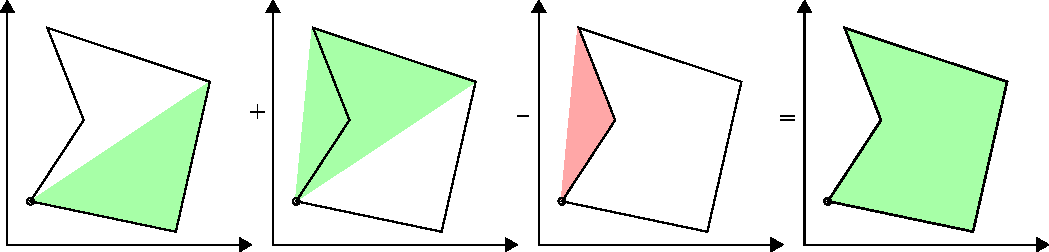
\includegraphics[width=\textwidth]{./img/ch5-area.pdf}
    \caption{A visual representation of the face area calculation algorithm. The area
    of the face is the sum of the areas of each triangle which can be build using the 
    pivot vertex and the other vertices of the face}
\end{figure}
\noindent
To compute the area of a generic (convex or concave) face,
we pick a pivot vertex of the face and then we iterate over
every edge of the face calculating the area of the triangle
made by the pivot vertex and the ordered extremes of the current edge.
The area of the full face is the sum of the areas of the single triangles.
This works because of the single triangles we compute the signed area with
this formula:
\begin{gather*}
    A = \frac{1}{2}
    \begin{vmatrix}
        p_{1x} & p_{1y} & 1 \\
        p_{2x} & p_{2y} & 1 \\
        p_{3x} & p_{3y} & 1
    \end{vmatrix}
\end{gather*}
Where $p_1$, $p_2$ and $p_3$ are the vertices of the triangle ($p_1$ is the pivot vertex). 
Please notice that the result of this formula will be negative only if these vertices 
are arranged in clockwise order.

@D Utilities
@{function face_area(V::Verts, EV::Cells, face::Cell)
    function triangle_area(triangle_points::Verts)
        ret = ones(3,3)
        ret[:, 1:2] = triangle_points
        return .5*det(ret)
    end

    area = 0

    fv = buildFV(EV, face)

    verts_num = length(fv)
    v1 = fv[1]

    for i in 2:(verts_num-1)

        v2 = fv[i]
        v3 = fv[i+1]

        area += triangle_area(V[[v1, v2, v3], :])
    end

    return area
end
@}

\subsection{Tests}
\begin{figure}[h]
    \centering
    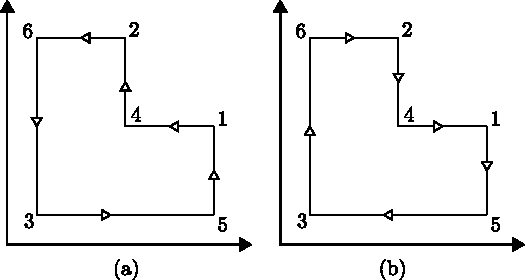
\includegraphics{./img/ch5-area_test.pdf}
\end{figure}
\noindent The two faces drawn above they must have complimentary area.
@D Utilities tests
@{@@testset "Face area calculation test" begin
    V = Float64[2 1; 1 2; 0 0; 1 1; 2 0; 0 2]
    EV = spzeros(Int8, 6, 6)
    EV[1, [1, 4]] = [-1, 1]; EV[2, [2, 4]] = [-1, 1]
    EV[3, [2, 6]] = [-1, 1]; EV[4, [3, 6]] = [-1, 1]
    EV[5, [3, 5]] = [-1, 1]; EV[6, [1, 5]] = [-1, 1]
    FE = spzeros(Int8, 2, 6)
    FE[1, :] = [ 1 -1  1 -1  1 -1]
    FE[2, :] = [-1  1 -1  1 -1  1]

    @@test LARLIB.face_area(V, EV, FE[1,:]) == -LARLIB.face_area(V, EV, FE[2,:])
end
@}

%%%%%%%%%%%%%%%%%%%%%%%%%%%%%%%%%%%%%
\section{External cell individuation}
\label{sec:external_cell}
To do this we iterate over the
vertices of the passed \texttt{EV} to find four vertices: the two with biggest
$x_1$ and $x_2$ coordinates (\texttt{maxv\_x1} and \texttt{maxv\_x2}) and the 
two with the smallest one (\texttt{minv\_x1} and \texttt{minv\_x2}). 
Then we check which face the two vertices have in common. 

It can happen that the two vertices have more than one face in common
(for example when a biconnected component is made up only by one face);
in this case we simply pick the cell with negative area. The area
computation routines are located into section \ref{sec:face_area},


@D Utilities
@{function get_external_cell(V::Verts, EV::Cells, FE::Cells)
    FV = abs.(FE)*EV
    vs = sparsevec(mapslices(sum, abs.(EV), 1)).nzind
    minv_x1 = maxv_x1 = minv_x2 = maxv_x2 = pop!(vs)
    for i in vs
        if V[i, 1] > V[maxv_x1, 1]
            maxv_x1 = i
        elseif V[i, 1] < V[minv_x1, 1]
            minv_x1 = i
        end
        if V[i, 2] > V[maxv_x2, 2]
            maxv_x2 = i
        elseif V[i, 2] < V[minv_x2, 2]
            minv_x2 = i
        end
    end
    cells = intersect(
        FV[:, minv_x1].nzind, 
        FV[:, maxv_x1].nzind,
        FV[:, minv_x2].nzind,
        FV[:, maxv_x2].nzind
    )
    if length(cells) == 1
        return cells[1]
    else
        for c in cells
            if face_area(V, EV, FE[c, :]) < 0
                return c
            end
        end
    end
end

function get_external_cell(V::Verts, EV::Cells, FE::Cells, CF::Cells)
    CV = abs.(CF)*abs.(FE)*EV
    vs = sparsevec(mapslices(sum, abs.(EV), 1)).nzind
    minv_x1 = maxv_x1 = minv_x2 = maxv_x2 = minv_x3 = maxv_x3 = pop!(vs)
    for i in vs
        if V[i, 1] > V[maxv_x1, 1]
            maxv_x1 = i
        elseif V[i, 1] < V[minv_x1, 1]
            minv_x1 = i
        end
        if V[i, 2] > V[maxv_x2, 2]
            maxv_x2 = i
        elseif V[i, 2] < V[minv_x2, 2]
            minv_x2 = i
        end
        if V[i, 3] > V[maxv_x3, 3]
            maxv_x3 = i
        elseif V[i, 3] < V[minv_x3, 3]
            minv_x3 = i
        end
    end
    cells = intersect(
        CV[:, minv_x1].nzind, 
        CV[:, maxv_x1].nzind,
        CV[:, minv_x2].nzind,
        CV[:, maxv_x2].nzind,
        CV[:, minv_x3].nzind,
        CV[:, maxv_x3].nzind
    )
    if length(cells) == 1
        return cells[1]
    else
        println("More than one cell found. Returning the first one.")
    end
end
@}

\subsubsection{Tests}
\begin{figure}[h]
    \centering
    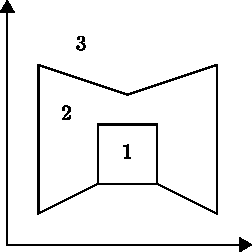
\includegraphics{./img/ch2-externcell.pdf}
    \caption{This biconnected component has three faces. The external one is the number 3.
    This is a particularly difficult case because the most "external" vertices of face 2
    are in common with the external cell.}
\end{figure}

@D Utilities tests
@{@@testset "External cell individuation" begin
    @@testset "d=2"
        V = [ .5 .5;  1.5   1;  1.5  2; 
            2.5  2;  2.5   1;  3.5 .5;
            3.5  3;    2 2.5;   .5  3]

        EV = Int8[-1  1  0  0  0  0  0  0  0;
                0 -1  1  0  0  0  0  0  0;
                0  0 -1  1  0  0  0  0  0;
                0  0  0 -1  1  0  0  0  0;
                0  0  0  0 -1  1  0  0  0;
                0  0  0  0  0 -1  1  0  0;
                0  0  0  0  0  0 -1  1  0;
                0  0  0  0  0  0  0 -1  1;
                -1  0  0  0  0  0  0  0  1;
                0 -1  0  0  1  0  0  0  0]
        EV = sparse(EV)
        
        FE = Int8[ 0 -1 -1 -1  0  0  0  0  0  1;
                1  1  1  1  1  1  1  1 -1  0;
                -1  0  0  0 -1 -1 -1 -1  1 -1]
        FE = sparse(FE)

        @@test LARLIB.get_external_cell(V, EV, FE) == 3
    end
    @@testset "d=3"
        V = [0 0 0; 1 0 0; 1 1 0; 0 1 0; 1 1 1] 

        EV = Int8[
            1 1 0 0 0;
            0 1 1 0 0;
            0 0 1 1 0;
            1 0 0 1 0;
            1 0 1 0 0;
            0 1 0 0 1;
            0 0 1 0 1;
            0 0 0 1 1;
            1 0 0 0 1]
        EV = sparse(EV)
        
        FE = Int8[
            1 1 0 0 1 0 0 0 0;
            0 0 1 1 1 0 0 0 0;
            0 1 0 0 0 1 1 0 0;
            0 0 1 0 0 0 1 1 0;
            0 0 0 0 1 0 1 0 1;
            0 0 0 1 0 0 0 1 1;
            1 0 0 0 0 1 0 0 1]
        FE = sparse(FE)

        CF = Int8[
            1 0 1 0 1 0 1;
            0 1 0 1 1 1 0;
            1 1 1 1 0 1 1]
        CF = sparse(CF)

        @@test LARLIB.get_external_cell(V, EV, FE, CF) == 3
    end
end
@}



%%%%%%%%%%%%%%%%%%%%%%%%
\section{Skeletal merge}
\label{sec:skel_merge}

The first step of the arrangement algorithm is ever
the skeletal merge [ref. \ref{sec:spatial_arrangement_overview}].

@D Utilities
@{function skel_merge(V1::Verts, EV1::Cells, V2::Verts, EV2::Cells)
    V = [V1; V2]
    EV = spzeros(Int8, EV1.m + EV2.m, EV1.n + EV2.n)
    EV[1:EV1.m, 1:EV1.n] = EV1
    EV[EV1.m+1:end, EV1.n+1:end] = EV2
    V, EV
end

function skel_merge(V1::Verts, EV1::Cells, FE1::Cells, V2::Verts, EV2::Cells, FE2::Cells)
    FE = spzeros(Int8, FE1.m + FE2.m, FE1.n + FE2.n)
    FE[1:FE1.m, 1:FE1.n] = FE1
    FE[FE1.m+1:end, FE1.n+1:end] = FE2
    V, EV = skel_merge(V1, EV1, V2, EV2)
    V, EV, FE
end
@}

%%%%%%%%%%%%%%%%%%%%%%%
\section{Edge deletion}
\label{sec:delete_edges}

Deleting edges ia a common operation in planar arrangement. When
edges are deleted, some vertices can remain unconnected; these must be deleted too.

@D Utilities
@{function delete_edges(todel, V::Verts, EV::Cells)
    tokeep = setdiff(collect(1:EV.m), todel)
    EV = EV[tokeep, :]
    
    vertinds = 1:EV.n
    todel = Array{Int64, 1}()
    for i in vertinds
        if length(EV[:, i].nzind) == 0
            push!(todel, i)
        end
    end

    tokeep = setdiff(vertinds, todel)
    EV = EV[:, tokeep]
    V = V[tokeep, :]

    return V, EV
end
@}


%%%%%%%%%%%%%%%%%%%%%%%
\section{FV building}

Sometimes is useful to represent a face like a sequence of vertices.

@D Utilities
@{function buildFV(EV::Cells, face::Cell)
    startv = -1
    nextv = 0
    edge = 0

    vs = Array{Int64, 1}()

    while startv != nextv
        if startv < 0
            edge = face.nzind[1]
            startv = EV[edge,:].nzind[face[edge] < 0 ? 2 : 1]
            push!(vs, startv)
        else
            edge = setdiff(intersect(face.nzind, EV[:, nextv].nzind), edge)[1]
        end
        nextv = EV[edge,:].nzind[face[edge] < 0 ? 1 : 2]
        push!(vs, nextv)

    end

    return vs[1:end-1]
end
@}


%%%%%%%%%%%%%%%%%%%%%%
\section{Boundaries building}

@D Utilities
@{function buildFE(FV, edges)
    faces = []

    for face in FV
        f = []
        for (i,v) in enumerate(face)
            edge = [v, face[i==length(face)?1:i+1]]
            ord_edge = sort(edge)

            edge_idx = findfirst(e->e==ord_edge, edges)

            push!(f, (edge_idx, sign(edge[2]-edge[1])))
        end
        
        push!(faces, f)
    end

    FE = spzeros(Int8, length(faces), length(edges))

    for (i,f) in enumerate(faces)
        for e in f
            FE[i, e[1]] = e[2]
        end
    end

    return FE
end

function buildEV(edges)
    maxv = max(map(x->max(x...), edges)...)
    EV = spzeros(Int8, length(edges), maxv)

    for (i,e) in enumerate(edges)
        e = sort(collect(e))
        EV[i, e] = [-1, 1]
    end

    return EV
end


function buildFV(EV::Cells, face)
    startv = face[1]
    nextv = startv

    vs = []
    visited_edges = []

    while true
        curv = nextv
        push!(vs, curv)

        edge = 0
        for edge in EV[:, curv].nzind
            nextv = setdiff(EV[edge, :].nzind, curv)[1]
            if nextv in face && (nextv == startv || !(nextv in vs)) && !(edge in visited_edges)
                break
            end
        end

        push!(visited_edges, edge)

        if nextv == startv
            break
        end
    end

    return vs
end


function build_bounds(edges, faces)
    EV = buildEV(edges)
    FV = map(x->buildFV(EV,x), faces)
    FE = buildFE(FV, edges)

    return EV, FE
end
@}


%%%%%%%%%%%%%%%%%%%%%
\section{Vertex equality utilities}
\label{sec:vertex_equality}

Vertex comparison must be performed using 
floating-point fixed error 
[ref. \ref{sec:floating-point_error}].

@D Utilities
@{function vin(vertex, vertices_set)
    for v in vertices_set
        if vequals(vertex, v)
            return true
        end
    end
    return false
end

function vequals(v1, v2)
    err = 10e-8
    return length(v1) == length(v2) && all(map((x1, x2)->-err < x1-x2 < err, v1, v2))
end
@}

%%%%%%%%%%%%%%%%%%%%%%%%%%%
\section{Full triangulation}


@D Utilities
@{function triangulate(V::Verts, EV::Cells, FE::Cells)

    triangulated_faces = Array{Any, 1}(FE.m)

    for f in 1:FE.m
        if f % 10 == 0
            print(".")
        end
        
        edges_idxs = FE[f, :].nzind
        edge_num = length(edges_idxs)
        edges = zeros(Int64, edge_num, 2)

        
        fv = buildFV(EV, FE[f, :])

        vs = V[fv, :]

        v1 = normalize(vs[2, :] - vs[1, :])
        v2 = [0 0 0]
        v3 = [0 0 0]
        err = 1e-8
        i = 3
        while -err < norm(v3) < err
            v2 = normalize(vs[i, :] - vs[1, :])
            v3 = cross(v1, v2)
            i = i + 1
        end
        M = reshape([v1; v2; v3], 3, 3)

        vs = (vs*M)[:, 1:2]
        
        for i in 1:length(fv)
            edges[i, 1] = fv[i]
            edges[i, 2] = i == length(fv) ? fv[1] : fv[i+1]
        end
        
        triangulated_faces[f] = TRIANGLE.constrained_triangulation(vs, fv, edges, fill(true, edge_num))

        tV = (V*M)[:, 1:2]
        
        area = face_area(tV, EV, FE[f, :])
        if area < 0 
            for i in 1:length(triangulated_faces[f])
                triangulated_faces[f][i] = triangulated_faces[f][i][end:-1:1]
            end
        end
    end

    return triangulated_faces
end
@}


%%%%%%%%%%%%%%%%%%%%%
\section{OBJ I/O}

OBj is a common format for 3D models exchange. 
Here an exporter of LAR model to OBJ. It returns a string.

@D Utilities
@{function lar2obj(V::Verts, EV::Cells, FE::Cells, CF::Cells)
    obj = ""
    for v in 1:size(V, 1)
        obj = string(obj, "v ", round(V[v, 1], 6), " ", round(V[v, 2], 6), " ", round(V[v, 3], 6), "\n")
    end

    print("Triangulating")
    triangulated_faces = triangulate(V, EV, FE)
    println("DONE")

    for c in 1:CF.m
    obj = string(obj, "\ng cell", c, "\n")
    for f in CF[c, :].nzind
        triangles = triangulated_faces[f]
        for tri in triangles
            t = CF[c, f] > 0 ? tri : tri[end:-1:1]
            obj = string(obj, "f ", t[1], " ", t[2], " ", t[3], "\n")
        end
    end
end

    return obj
end
@}

And here an importer. It wants a path to the obj file
expressed as a string. It returns the classic tuple \texttt{V, EV, FE}.

@D Utilities
@{function obj2lar(path)
    fd = open(path, "r")
    vs = Array{Float64, 2}(0, 3)
    edges = Array{Array{Int, 1}, 1}()
    faces = Array{Array{Int, 1}, 1}()

    while (line = readline(fd)) != ""
        elems = split(line)
        if length(elems) > 0
            if elems[1] == "v"

                x = parse(Float64, elems[2])
                y = parse(Float64, elems[3])
                z = parse(Float64, elems[4])
                vs = [vs; x y z]

            elseif elems[1] == "f"
                v1 = parse(Int, elems[2])
                v2 = parse(Int, elems[3])
                v3 = parse(Int, elems[4])

                e1 = sort([v1, v2])
                e2 = sort([v2, v3])
                e3 = sort([v1, v3])

                if !(e1 in edges)
                    push!(edges, e1)
                end
                if !(e2 in edges)
                    push!(edges, e2)
                end
                if !(e3 in edges)
                    push!(edges, e3)
                end

                push!(faces, sort([v1, v2, v3]))
            end
        end
    end

    close(fd)
    vs, build_bounds(edges, faces)...
end  
@}


%%%%%%%%%%%%%%%%%%%%%%
\section{Point in face area}
\label{sec:point_in_face}

Point in face inclusion is performed using the algorithm
presented by A. Paoluzzi in 1986 \cite{Paoluzzi-ART1986}.
It is based on the ray shooting and it analyzes more than
thirty possible ray-edge intersection cases.

@D Utilities
@{function point_in_face(origin, V::Verts, ev::Cells)

    function pointInPolygonClassification(V,EV)

        function crossingTest(new, old, status, count)
        if status == 0
            status = new
            return status, (count + 0.5)
        else
            if status == old
                return 0, (count + 0.5)
            else
                return 0, (count - 0.5)
            end
        end
        end

        function setTile(box)
        tiles = [[9,1,5],[8,0,4],[10,2,6]]
        b1,b2,b3,b4 = box
        function tileCode(point)
            x,y = point
            code = 0
            if y>b1 code=code|1 end
            if y<b2 code=code|2 end
            if x>b3 code=code|4 end
            if x<b4 code=code|8 end
            return code
        end
        return tileCode
        end

        function pointInPolygonClassification0(pnt)
            x,y = pnt
            xmin,xmax,ymin,ymax = x,x,y,y
            tilecode = setTile([ymax,ymin,xmax,xmin])
            count,status = 0,0

            for k in 1:EV.m
                edge = EV[k,:]
                p1, p2 = V[edge.nzind[1], :], V[edge.nzind[2], :]
                (x1,y1),(x2,y2) = p1,p2
                c1,c2 = tilecode(p1),tilecode(p2)
                c_edge, c_un, c_int = xor(c1, c2), c1|c2, c1&c2
                
                if (c_edge == 0) & (c_un == 0) return "p_on" 
                elseif (c_edge == 12) & (c_un == c_edge) return "p_on"
                elseif c_edge == 3
                    if c_int == 0 return "p_on"
                    elseif c_int == 4 count += 1 end
                elseif c_edge == 15
                    x_int = ((y-y2)*(x1-x2)/(y1-y2))+x2 
                    if x_int > x count += 1
                    elseif x_int == x return "p_on" end
                elseif (c_edge == 13) & ((c1==4) | (c2==4))
                        status, count = crossingTest(1,2,status,count)
                elseif (c_edge == 14) & ((c1==4) | (c2==4))
                        status, count = crossingTest(2,1,status,count)
                elseif c_edge == 7 count += 1
                elseif c_edge == 11 count = count
                elseif c_edge == 1
                    if c_int == 0 return "p_on"
                    elseif c_int == 4 
                        status, count = crossingTest(1,2,status,count) 
                    end
                elseif c_edge == 2
                    if c_int == 0 return "p_on"
                    elseif c_int == 4 
                        status, count = crossingTest(2,1,status,count) 
                    end
                elseif (c_edge == 4) & (c_un == c_edge) return "p_on"
                elseif (c_edge == 8) & (c_un == c_edge) return "p_on"
                elseif c_edge == 5
                    if (c1==0) | (c2==0) return "p_on"
                    else 
                        status, count = crossingTest(1,2,status,count) 
                    end
                elseif c_edge == 6
                    if (c1==0) | (c2==0) return "p_on"
                    else 
                        status, count = crossingTest(2,1,status,count) 
                    end
                elseif (c_edge == 9) & ((c1==0) | (c2==0)) return "p_on"
                elseif (c_edge == 10) & ((c1==0) | (c2==0)) return "p_on"
                end
            end
            
            if (round(count)%2)==1 
                return "p_in"
            else 
                return "p_out"
            end
        end
        return pointInPolygonClassification0
    end
    
    return pointInPolygonClassification(V, ev)(origin) == "p_in"
end
@}